\documentclass{article}
\usepackage[OT1]{fontenc}
\usepackage{graphicx}
\usepackage{setspace}
\usepackage{anysize}
\usepackage{enumerate}
\usepackage{amssymb}
\usepackage{algorithm2e}
\usepackage{amsthm}
\usepackage{amsmath}
\usepackage{booktabs}
\usepackage{ulem}
\marginsize{3cm}{3cm}{0cm}{3cm}

\fontfamily{ptm}\fontsize{14}{14}\selectfont 
\singlespacing
\newcommand{\solution}[1]{~\\ $\blacksquare$ \sffamily\upshape\selectfont #1
\normalfont ~\\~ }
\newcommand\independent{\protect\mathpalette{\protect\independenT}{\perp}}
\def\independenT#1#2{\mathrel{\rlap{$#1#2$}\mkern2mu{#1#2}}} 
\setlength{\parindent}{0pt}
% \setlength{\textwidth}{1.5\textwidth}

\begin{document}
\begin{center}
\textbf{\large{
HOMEWORK 2 \\
Introduction to Artifitial Intelligence \\}}
\textsc{\Large{Shumin Guo}}
\end{center}

\section{Execise 13.7}
Consider the set of all possible five-card poker hands dealt fairly
from a standard deck of fifty-two cards.
\begin{enumerate}[a.]
\item How many atomic events are there in the joint probability
  distribution (i.e., how many five-card hands are there)?
  \solution{Since the order of hands does not matter, the total number
  of hands is a combination of all possiblities choosing five cards
  from fifty-two cards. 
  \[ {52 \choose 5} = \frac{52!}{5!\times (52-5)!} =
  \frac{8.06581752\times 10^{67}}{120\times 2.58623242 \times 10^{59}}
  = 2,598,960. \]
} 
\item What is the probability of each atomic event?
  \solution{Considering that all the atomic events will happen with
    equal probability, we can get the probability of one atomic event
    as \[ \frac{1}{2,598,960}=3.84769292\times 10^{-7}. \]} 
\item What is the probability of being dealt a royal straight flush?
  Four of a kind? 
  \solution{A royal straight flush means the combination of A,K,Q,J
    and 10 with the same type. So there are totally four royal
    straight flushes shown as below. 
    \[ A(\clubsuit), K(\clubsuit), Q(\clubsuit), J(\clubsuit),
    10(\clubsuit) \] 
    \[ A(\spadesuit), K(\spadesuit), Q(\spadesuit), J(\spadesuit),
    10(\spadesuit) \]
    \[ A(\heartsuit), K(\heartsuit), Q(\heartsuit), J(\heartsuit),
    10(\heartsuit) \]
    \[ A(\diamondsuit), K(\diamondsuit), Q(\diamondsuit), J(\diamondsuit),
    10(\diamondsuit) \]
    
    And the possibility of being dealt a royal straight flush is 
    \[ \frac{4}{2,598,960}=1.53907717 \times 10^{-6}. \] 
  }
\end{enumerate}

\section{Execise 13.11}
We wish to transmit an $n$-bit message to a receiving agent. The bits
in the message are independently corrupted (flipped) diming
transmission with $\epsilon$ probability each. With an extra parity
bit sent along with the original information, a message can be
corrected by the receiver if at most one bit in the entire message
(including the parity bit) has been corrupted. Suppose we want to
ensure that the correct message is received with probability at least
$1-\delta$. What is the maximum feasible value of $n$? Calculate this
value for the case $\epsilon = 0.001, \delta = 0.01$.
\solution{
  In order to make sure the probability of received message to be at
  least $1-\delta$, we need to make sure that the total probability of
  have one-bit error and have zero-bit error to be $1-\delta$. \\
  Let's suppose the probability of have 1-bit error is $P(1)$ and 0-bit
  error is $P(0)$. We have 
  \[ P(0) = {n+1 \choose 0}\times \epsilon ^{0}\times (1-\epsilon)^{n+1}
  = (1-\epsilon)^{n+1} \]
  \[ P(1) = {n+1 \choose 1}\times \epsilon ^{1}\times (1-\epsilon)^{n}
  = (n+1)\times \epsilon \times (1-\epsilon)^n \]
  and the maximum acceptable total error rate is: 
  \[ P(0) + P(1) = 1 - \delta \]
\begin{eqnarray*}
  (1+n\epsilon)(1-\epsilon)^n & = & 1-\delta \\
  \mbox{for } \epsilon = 0.001, \mbox{ and } \delta =  0.01, && \\
  (1+0.001n)(1-0.001)^n & = & 1-0.01 \\
  (1+0.001n)0.999^n & = & 0.99  \\
  n & \approx & 148. 
\end{eqnarray*}
  So, the maximum feasible value of $n$ is approximately 148. 
}
\section{Execise 13.17}
Show that the statement of conditional independence
\[ P(X,Y|Z)=P(X|Z)P(Y|Z) \]
is equivalent to each of the statements
\[ P(X|Y,Z)=P(X|Z) \mbox{ and } P(Y|X,Z)=P(Y|Z). \]
\solution{
  For equivalence of $P(X,Y|Z)=P(X|Z)P(Y|Z) \mbox{ and }
  P(X|Y,Z)=P(X|Z)$:  \\  
  (a) $P(X,Y|Z)=P(X|Z)P(Y|Z) \Longrightarrow P(X|Y,Z)=P(X|Z)$:
  \begin{eqnarray*}
    P(X,Y|Z) & = & P(X|Z)P(Y|Z) \\ 
    \frac{P(X,Y,Z)}{P(Z)} & = & P(X|Z)P(Y|Z) \\
    P(X|Y,Z)P(Y|Z) & = & P(X|Z)P(Y|Z) \\
    P(X|Y,Z) & = & P(X|Z)
  \end{eqnarray*}
  (b) $P(X|Y,Z)=P(X|Z) \Longrightarrow P(X,Y|Z)=P(X|Z)P(Y|Z)$: 
  \begin{eqnarray*}
    P(X|Y,Z) & = & P(X|Z) \\ 
    \frac{P(X,Y,Z)}{P(Y,Z)} & = & P(X|Z) \\
    \frac{P(X,Y|Z)}{P(Y|Z)} & = & P(X|Z) \\ 
    P(X,Y|Z) & = & P(X|Z)P(Y|Z)
  \end{eqnarray*}
  
  For evalence of $P(X,Y|Z)=P(X|Z)P(Y|Z) \mbox{ and }
  P(Y|X,Z)=P(Y|Z)$: \\   
  (a) $P(X,Y|Z)=P(X|Z)P(Y|Z) \Longrightarrow P(Y|X,Z)=P(Y|Z)$:  
  \begin{eqnarray*}
    P(X,Y|Z) & = & P(X|Z)P(Y|Z) \\
    \frac{P(X,Y,Z)}{P(Z)} & = & P(X|Z)P(Y|Z) \\
    P(Y|X,Z)P(X|Z) & = & P(X|Z)P(Y|Z) \\
    P(Y|X,Z) & = & P(Y|Z) 
  \end{eqnarray*}
  (b) $P(Y|X,Z)=P(Y|Z) \Longrightarrow P(X,Y|Z)=P(X|Z)P(Y|Z)$:  
  \begin{eqnarray*}
    P(Y|X,Z) & = & P(Y|Z) \\
    \frac{P(X,Y|Z)}{P(X|Z)} & = & P(Y|Z) \\
    P(X,Y|Z) & = & P(X|Z)P(Y|Z) 
  \end{eqnarray*}
}
\section{Execise 13.18}
Suppose you are given a bag containing $n$ unbiased coins. You are told
that $n-1$ of these coins are normal, with heads on one side and tails
on the other, whereas one coin is a fake, with heads on both sides.
\begin{enumerate}[a.]
  \item Suppose you reach into the bag, pick out a coin at random,
    flip it, and get a head, What is the (conditional) probability that
    the coin you chose is the fake coin?
    \solution{Let's use $H$ to denote head, $T$ to denote tail,
      $C_{normal}$ to denote normal coin and $C_{fake}$ to denote fake
      coin. Because all the coins are unbiased, we can calculate the
      prior probability as follows:  
      \begin{eqnarray*}
        P(C_{normal}) & = & \frac{n-1}{n} \\ 
        P(C_{fake}) & = & \frac{1}{n} \\
        P(H|C_{normal}) & = & 0.5 \\ 
        P(T|C_{normal}) & = & 0.5 \\
        P(H|C_{fake}) & = & 1 \\ 
        P(T|C_{fake}) & = & 0
      \end{eqnarray*}
      By using the above prior probabilities we can calculate the
      following probabilities: 
      \begin{eqnarray*}
        P(H) & = & P(H|C_{normal})P(C_{normal}) + P(H|C_{fake})P(C_{fake})  \\
        & = & 0.5\times \frac{n-1}{n} + 1\times \frac{1}{n} \\
        & = & \frac{0.5(n+1)}{n} \\
      \end{eqnarray*}
      And, the probability of choosing a fake coin after getting
      head from a random chosen coin toss can be represented by
      $P(C_{fake}|H)$. And we have: 
      \begin{eqnarray*}
        P(C_{fake}|H) & = & \frac{P(H|C_{fake})P(C_{fake})}{P(H)} \\
        & = & \frac{1\times \frac{1}{n}}{\frac{0.5(n+1)}{n}} \\
        & = & \frac{2}{n+1}
      \end{eqnarray*}
} 
  \item Suppose you continue flipping the coin for a total of $k$ times
    after picking it and see $k$ heads. Now what is the conditional
    probability that you picked the fake coin?
    \solution{The conditional probability of getting of fake coin can
      be represented as $P(C_{fake}|\overbrace{H,\ldots,H}^\text{total
        k Hs})$. \\
      And by using Baysian rule, we have: \\
      \begin{eqnarray*}
        P(C_{fake}|\overbrace{H,\ldots,H}^\text{total k Hs}) & = &
        \frac{P(C_{fake},\overbrace{H,\ldots,H}^\text{total k
            Hs})}{P(\underbrace{H,\ldots,H}_\text{total k Hs})} \\
        & = & \frac{\prod_{i=1}^k P(H|C_{fake})P(C_{fake})}
        {P(\underbrace{H,\ldots,H}_{\mbox{total k Hs}}|C_{normal})P(C_{normal}) 
          + P(\underbrace{H,\ldots,H}_{\mbox{total k Hs}}|C_{fake})P(C_{fake})} \\
        & = & \frac{P(C_{fake})}{{k \choose
            k}P(H|C_{normal})^kP(T|C_{normal})^0 + {k \choose
            k}P(H|C_{fake})^kP(T|C_{fake})^0}  \\
        & = & \frac{\frac{1}{n}}{0.5^k\frac{n-1}{n}+1^k\frac{1}{n}} \\
        & = & \frac{1}{0.5^k(n-1)+1} \\
        & = & \frac{2^k}{2^k+n-1}
      \end{eqnarray*}
} 
  \item Suppose you wanted to decide whether the chosen coin was fake by
    flipping it $k$ times.  The decision procedure returns $fake$ if all $k$
    flips come up heads; otherwise it returns $normal$. What is the
    (unconditional) probability that this procedure makes an error?
    \solution{Error will happen when the randomly picked coin is
      actually a normal coin rather than a fake one when we get $k$
      heads. So, it can be represented with
      $P(C_{normal}|\overbrace{H,\ldots,H}^{\mbox{total k Hs}})$.

      By using the result from the last equestion, we can calculate
      the error rate as: \\
      \begin{eqnarray*}
        P(C_{normal}|\overbrace{H,\ldots,H}^{\mbox{total k Hs}}) & = & 
        1 - P(C_{fake}|\overbrace{H,\ldots,H}^{\mbox{total k Hs}}) \\
        & = & 1 - \frac{2^k}{2^k+n-1} \\
        & = & \frac{n-1}{2^k+n-1}
      \end{eqnarray*}
      This result tells us that given finite number of coins $n$, when
      $k$ is larger, the error rate will become smaller. 
    }
\end{enumerate}
\section{Execise 13.21}
(Adapted from Pearl (1988).) Suppose you are a witness to a nighttime
hit-and-run accident involving a taxi in Athens. All taxis in Athens
are blue or green. You swear, under oath, that the taxi was
blue. Extensive testing shows that, under the dim lighting conditions,
discrimination between blue and green is $75\%$ reliable.
\begin{enumerate}[a.]
\item Is it possible to calculate the most likely color for the taxi?
  (Hint: distinguish carefully between the proposition that the taxi is
  blue and the proposition that it appears blue.)
  \solution{According to the description of the problem, let's use $B$
    to denote blue taxi, $G$ to denote green taxi, $LB$ to denote taxi
    that is likely blue and $LG$ to denote taxi that is likely green,
    we can have prior probabilities as follows: \\ 
    \begin{eqnarray*}
      \mbox{Prior probability of blue and green is unknow: } \\
      P(B) & = & ? \\
      P(G) & = & ? \\
      \mbox{Discrimination between Blue and Green: } \\
      P(LB|B) & = & 0.75 \\ 
      P(LG|B) & = & 0.25 \\
      P(LG|G) & = & 0.75 \\
      P(LB|G) & = & 0.25
    \end{eqnarray*}
    So, the likely color for the taxi can be reprented as $P(B|LB)$. 
    And according to bayes rule, we have: \\ 
    \[ P(B|LB)=\frac{P(LB|B)P(B)}{P(LB)} \]
    In order to calculate this formula, we need to know the prior
    probability of $P(B)$, which is not given, so it is impossible to
    calculate the most likely color for the taxi. 
  }
\item What if you know that 9 out of 10 Athenian taxis are green?
  \solution{Now, we have $P(B)=0.1$ and $P(G)=0.9$. And we can
    calculate the probability of the most likely color of taxi as
    follows: \\ 
    \begin{eqnarray*}
      P(B|LB) & = & \frac{P(LB|B)P(B)}{P(LB)} \\
      & = & \frac{P(LB|B)P(B)}{P(LB|B)P(B) + P(LB|G)P(G)} \\
      & = & \frac{0.75\times 0.1}{0.75\times 0.1 + 0.25\times 0.9} \\
      & = & \frac{0.075}{0.075+0.225} \\ 
      & = & \frac{0.075}{0.3} \\
      & = & 0.25 \\ 
      \mbox{So, we have: } P(G|LB) & = & 1-P(B|LB) \\
      & = & 1-0.25 \\
      & = & 0.75
    \end{eqnarray*}
  }
\end{enumerate}
\section{Execise 13.22}
Text categorization is the task of assigning a given document to one
of a fixed set of categories on the basis of the text it
contains. Naive Bayes models are often used for this task. In these
models, the query variable is the document category, and the "effect"
variables are the presence or absence of each word in the language;
the assumption is that words occur independently in documents, with
frequencies determined by the document category.
\begin{enumerate}[a.]
\item Explain precisely how such a model can be constructed, given as
  "training data" a set of documents that have been assigned to
  categories.
  \solution{
    The probability model of a document classifier can be represented
    with a conditional model $p(c|f_1,f_2,\ldots,f_n)$, where $c$ is
    class variable of document, $f_1\ldots, f_n$ is vector of features,
    for example, words that appear in documents. \\
    Using Bayes's theorem, we have: \\
    \[ p(c|f_1,f_2,\ldots,f_n) =
    \frac{p(c)p(f_1,f_2,\ldots,f_n|c)}{p(f_1,f_2,\ldots, f_n)} \]
    By means of Naive Bayes model, we can rewrite the above formula to
    be 
    \[ p(c|f_1,f_2,\ldots,f_n) =
    \frac{p(c)\prod_{i=1}^np(f_i|c)}{p(f_1,f_2,\ldots, f_n)} \]
    since the denominator does not depend on class $c$, and the value of
    features are given by training data set, which means that the
    denominator is constant as far as the classifier is concerned,
    so, we can ignore the denominator, and the final classifier is 
    \[ p(c|f_1,f_2,\ldots,f_n) \propto p(c)\prod_{i=1}^np(f_i|c). \]

    In text classification, our goal is to find the best class for a given
    document, and the best class in Naive bayesian classification is
    the most likely or maximum a posteriori(MAP) class $c_{map}$. And 
    \[ c_{map} = \arg\max_{c\in C}\hat{p}(c|d)=\arg\max_{c\in
      C}\hat{p}(c)\prod_{1\leq i \leq n}\hat{p}(f_i|c). \]
    And usually, it is easier for us to compute the log likelihood of
    the above formula, due to the fact that logarithm function is
    monotonically increasing function. So the maximization of MAP can
    be written as 
    \[ c_{map}=\arg\max_{c\in C}[\mbox{log}\hat{p}(c)+\sum_{1\leq i \leq
      n}\mbox{log}\hat{p}(f_i|c)]. \]
    It is not possible to know the true values of $p(c)$ and
    $p(f_i|c)$, but we can estimate their values from the given
    training data sets. 

    $p(c)$ indicates the relative frequency of class $c$, more
    frequent classes are more likely to be the correct class than
    infrequent classes. The sum of log prior and term weights is a
    measure of how much evidence there is for the document being in
    the class. So we have the following estimates for both part. 
    \[ \hat{p}(c)=\frac{N_c}{N} \]
    where $N_c$ is total number of documents in class $c$ and $N$ is
    the total number of documents. \\ 
    And similarly, the conditional probability $\hat{p}(f|c)$ can be
    estimated as the relative frequency of feature (here are words)
    $f$ in documents belonging to class $c$. 
    \[ \hat{p}(t|c)=\frac{N_{cf}}{\sum_{f^{\prime}\in F}N_{cf^{\prime}}} \]
    where $N_{cf}$ is count of occurences of feature $f$ occurs in
    class $c$, and $\sum_{f^{\prime}\in F}N_{cf^{\prime}}$ is count of all the
    features that occur in class $c$. 

    In summary and technically, in order to build this naive bayesian
    classifier using the given training data set, we need to do the
    following things.  \\ 
    \begin{enumerate}
    \item Extract a bag of words that appear in training data set. 
    \item Count total docs and docs that occur in class $c$. 
    \item Count occurrances of words in each class. 
    \item Calculate the prior probability of $\hat{p}(c)$ and
      $\hat{p}(f_i|c)$. 
    \item Calculate log-summed posterior probability using
      $[\mbox{log}\hat{p}(c)+\sum_{1\leq i \leq
        n}\mbox{log}\hat{p}(f_i|c)]$. 
     \end{enumerate}
  }
\item Explain precisely how to categorize a new document. 
  \solution{To categorize a new document, we need to follow steps
    below: \\ 
  \begin{itemize}
    \item Extract words from new document. 
    \item Calculate logged prior probability of $\hat{p}(c)$ for each class
      $c$. 
    \item Calculate logged sum conditional probability of words using
      $\sum_{1\leq i \leq n}\mbox{log}\hat{p}(f_i|c)$ for each class. 
    \item Return the class that can maximize $p(c|f_1,f_2,\ldots,f_n)$,
      which is the most likely class of the new document based on the
      training data set. 
  \end{itemize}
}
\item Is the conditional independence assumption reasonable? Discuss. 
  \solution{In reality, the conditional independence does not hold for text
  data, terms are conditionally dependent on each other. But in fact
  the Naive Bayesian classifier can perform really good. The reasons
  are that NB classification does not use estimated probability to
  make decision, rather, it uses the relative estimated probability to
  make the decision. So, even though it might have a bad estimate with the
  independence assumption, it can always estimates correct relative
  probability over all classes. Thus, although estimate badly, NB
  classifiers can classify very well. }
\end{enumerate}
\section{Execise 14.1}
We have a bag of three biased coins $a$, $b$. and $c$ with
probabilities of coming up heads of $20\%, 60\%$, and $80\%$,
respectively. One coin is drawn randomly from the bag (with equal
likelihood of drawing each of the three coins), and then the coin is
flipped three times to generate the outcomes $X_1$, $X_2$, and $X_3$.
\begin{enumerate}[a.]
\item Draw the Bayesian network corresponding to this setup and define
  the necessary CPTs. 
  \solution{
    Please see Bayesian network in Figure \ref{fig:14_1}. It is
    obvious that $X_1,X_2 \mbox{ and } X_3$ are independent events
    with the same probability for head(H) and tail(T) and thus
    can be represented with a single node (Flip Result) to denote,
    without any interaction among the three variables. 
    \begin{figure}[ht]
      \centering
      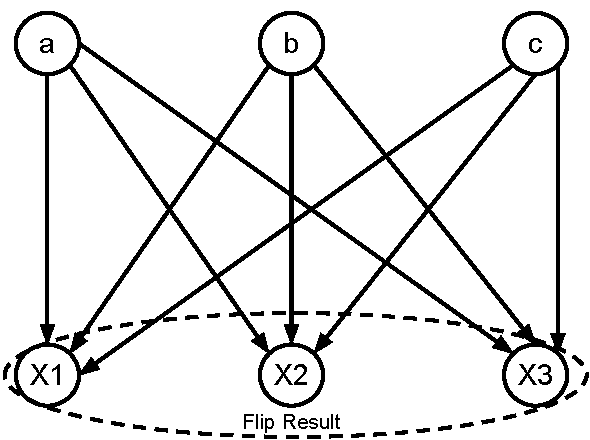
\includegraphics[width=.5\textwidth]{AI-HWK-2_14_1.pdf}
      \caption{Bayesian Network for coin flipping.}\label{fig:14_1}
    \end{figure}
    Please find the CPT in Table \ref{tbl:ai-hwk2-14-1}. Note that,
    because $X_1,X_2,X_3$ have the same probability tables, so, only
    the CPT of $X_1$ is listed. 
  \begin{table}[h]
    \centering
    \begin{tabular}{l|l}
      \toprule
      \textbf{Probability} & \textbf{Value} \\ \toprule
      $P(a)$ & $\frac{1}{3}$ \\ \midrule
      $P(b)$ & $\frac{1}{3}$ \\ \midrule
      $P(c)$ & $\frac{1}{3}$ \\ \midrule
      $P(X_1=H|a)$ & 0.2 \\ \midrule
      $P(X_1=T|a)$ & 0.8 \\ \midrule
      $P(X_1=H|b)$ & 0.6 \\ \midrule
      $P(X_1=T|b)$ & 0.4 \\ \midrule 
      $P(X_1=H|c)$ & 0.8 \\ \midrule 
      $P(X_1=T|c)$ & 0.2 \\
      \bottomrule
    \end{tabular}
    \caption{CPT for Bayesian Network.}
    \label{tbl:ai-hwk2-14-1}
  \end{table}
  }
\item Calculate which coin was most likely to have been drawn from the
  bag if the observed flips come out heads twice and tails once.
  \solution{
    We can calculate the estimated probability with the given
    information $P(H)=\frac{2}{3} \mbox{ and } P(T)=\frac{1}{3}$. We
    need to calculate the posterior probability of three types of coin
    using the given evidence probability. 
    \[ P(C|H,H,T) \] where $C$ is type of coin, which can be $a,b
    \mbox{ and } c$. We can rewrite the probability based on bayesian
    and independence rule as \[ P(C|H,H,T) = \frac{P(H,H,T|C)P(C)}{P(H,H,T)} =
    \frac{P(H|C)P(H|C)P(T|C)P(C)}{P(H,H,T)}. \]
    Because denominator $P(H,H,T)$ is independent of class, and will
    be a constant value for all three classes upon given evidence, we
    can simply ignore it. So, \[ P(C|H,H,T) \propto P(H|C)P(H|C)P(T|C)P(C). \]
    Then, we can calculate the posterior probability for each class as
    \begin{eqnarray*}
      P(a|H,H,T) \propto P(H|a)P(H|a)P(T|a)P(a) & = &
      0.2\times 0.2\times 0.8 \times \frac{1}{3} \approx 0.0107 \\
      P(b|H,H,T) \propto P(H|b)P(H|b)P(T|b)P(b) & = &
      0.6\times 0.6\times 0.4 \times \frac{1}{3} = 0.048 \\
      P(c|H,H,T) \propto P(H|c)P(H|c)P(T|c)P(c) & = &
      0.8\times 0.8\times 0.2 \times \frac{1}{3} \approx 0.0427 
    \end{eqnarray*}
    It is obvious that $P(b|H,H,T)$ has the maximum probability among
    three types of coins, so, coin $b$ is the most likely coin to have
    been drawn from the bag. 
  }
\end{enumerate}
\section{Execise 14.4}
Consider the Bayesian network in Figure \ref{fig:1}.
% figure 14.2. 
\begin{figure}[ht]
  \centering
  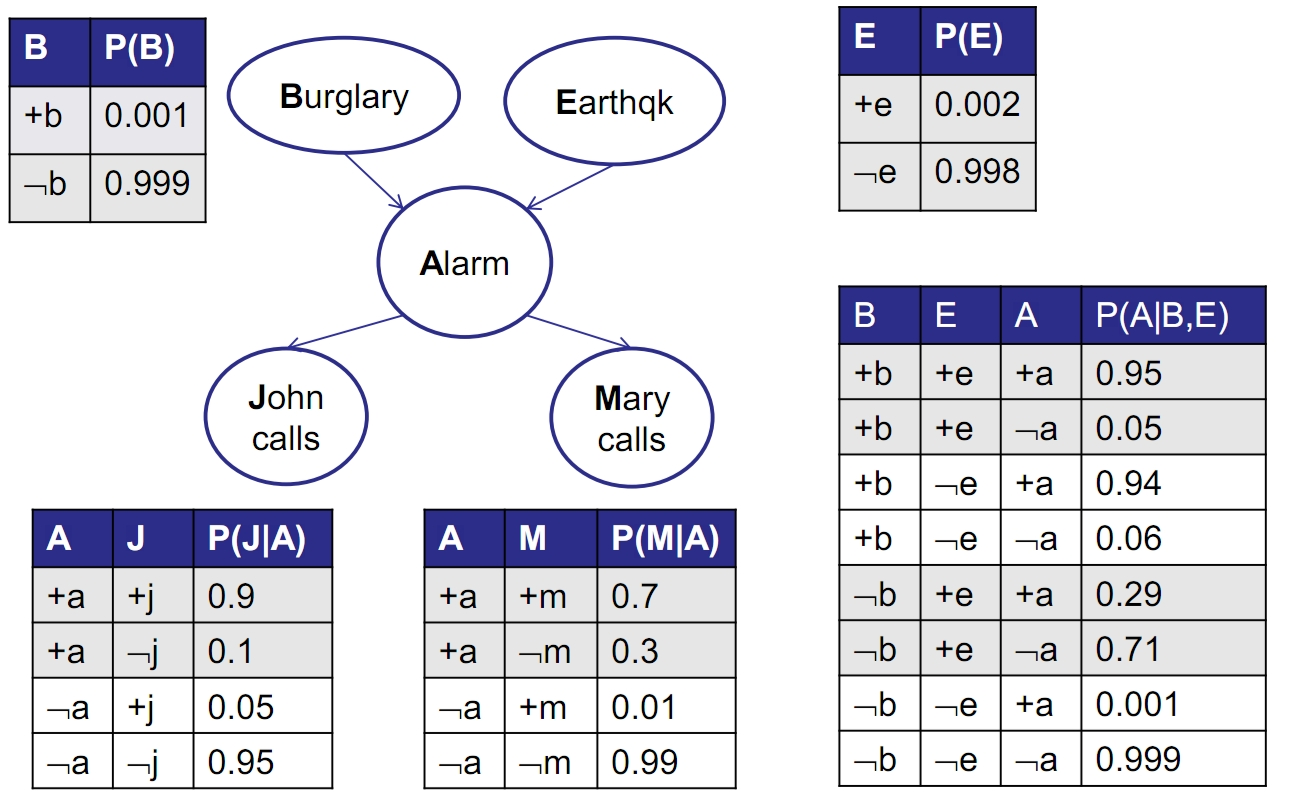
\includegraphics[width=.6\textwidth]{fig14_2.jpg}
  \caption{A typical Bayesian network, showing both the topology and
    the conditional probability tables (CPTs). In the CPTs, the
    letters B, E, A, J, and M stand for $Burglary, Earthquake,
    Alarm, John Calls,$ and $MaryCalls$, respectively. 
  }
  \label{fig:1}
\end{figure}
\begin{enumerate}[a.]
\item If no evidence is observed, are Burglary and Earthquake
  independent? Prove this from the numerical semantics and from the
  topological semantics.
  \solution{Yes, they are independent if no evidence is observed. \\ 
    For numerical semantics, we have 
    \begin{eqnarray*}
      P(Burglary, Earthquake) & = &
      P(Burglary|parents(Burglary))P(Earthquake|parents(Earthquake))  \\
  & = & P(Burglary)P(Earthquake). 
\end{eqnarray*}
So, Burglary and Earthquake are independent. \\
The topological semantics specifies that each variable is
conditionally independent of its non-descendants, given its
parents. As can be seen from Figure \ref{fig:1}, Burglary is
non-decendant of Earthquake, thus they are independent in
topological semantics. 
}
\item If we observe Alarm=true, are Burglary and Earthquake
independent? Justify your answer by calculating whether the
probabilities involved satisfy the definition of conditional
independence.
\solution{No, they are not independent. \\
We need to test if $P(B,E|A) = P(B|A)P(E|A)$ holds. 
\begin{eqnarray*}
P(A) & = & P(A|B,E)P(B)P(E) + P(A|B,\neg E)P(B)P(\neg E) \\ 
& + & P(A|\neg B,E)P(\neg B)P(E) + P(A|\neg B,\neg E)P(\neg B)P(\neg E) \\ 
& = & 0.95\times 0.001\times 0.002 + 0.94\times 0.001\times 0.998 +
0.29\times 0.999\times 0.002 + 0.001\times 0.999 \times 0.998 \\ 
& = & 0.0000019 + 0.00093812 + 0.00057942 + 0.00098901 = 0.00251 \\
P(B|A) & = & \frac{P(A|B)P(B)}{P(A)} 
= \frac{P(A|B,E)P(B)P(E)+P(A|B,\neg E)P(B)P(\neg E)}{P(A)} \\
& = & \frac{0.95\times 0.001\times 0.002 + 0.94\times 0.001\times
  0.998}{0.00251}\\ 
& = & \frac{0.00094002}{0.00251} = 0.37451 \\
P(E|A) & = & \frac{P(A,E)}{P(A)}
 = \frac{P(A,E|B)P(B)+P(A,E|\neg B)P(\neg B)}{P(A)} \\
& = & \frac{P(A|B,E)P(B)P(E)+P(A|\neg B,E)P(\neg B)P(E)}{P(A)} \\
& = & \frac{0.95\times 0.001\times 0.002 + 0.29\times 0.999\times
  0.002}{0.00251} \\ 
& = & \frac{0.00058132}{0.00251} = 0.2316 \\
P(B|A)P(E|A) & = & 0.37451 \times 0.2316 = 0.0867 \\
P(B,E|A) & = & \frac{P(A|B,E)P(B,E)}{P(A)}
 = \frac{P(A|B,E)P(B)P(E)}{P(A)} = \frac{0.95\times 0.001\times 0.002}{0.00251} = 0.000757 
\end{eqnarray*}
So, it is clear that $P(B,E|A)\neq P(B|A)P(E|A)$, which means they are
not independent given Alarm = true. 
}
\end{enumerate}
\section{Execise 14.11}
In your local nuclear power station, there is an alarm that senses
when a temperature gauge exceeds a given threshold. The gauge measures
the temperature of the core. Consider the Boolean variables A (alarm
sounds), $F_A$ (alarm is faulty), and $F_G$ (gauge is faulty) and the
multivalued nodes G (gauge reacting) and T (actual core temperature).
\begin{enumerate}[a.]
\item Draw a Bayesian network for this domain, given that the gauge is
  more likely to fail when the core temperature gets too high.
\solution{
  Please find the bayesian network in Figure \ref{fig:3}. 
  % solution for the bayesian network. 
  \begin{figure}[ht]
    \centering
    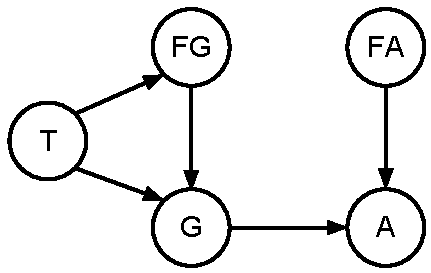
\includegraphics[width=.3\textwidth]{AI-HWK-2_14_11.pdf}
    \caption{Bayesian Network for nuclear power station alarm system.} 
    \label{fig:3}
  \end{figure} }
\item Is your network a polytree? Why or why not?
\solution{No, this is not a polytree structure, because there is a loop
structure formed by three nodes: $T, G, FG$, which makes it no a tree
structure any more. }
\item Suppose there are just two possible actual and measured
  temperatures, normal and high; the probability that the gauge gives
  the correct temperature is $x$ when it is working, but $y$ when it is
  faulty. Give the conditional probability table associated with G.
  \solution{Let's use $T$ to denote normal temperature, $\neg T$ to
    denote high temperature, $G$ to denote guage works normally, and
    $\neg G$ to denote gauge works abnormally; $F_G$ denote guage
    fault and $\neg F_G$ to denote guage non-fault. 
    Please see the CPT in Table \ref{tbl:ai-hwk2-14-11.1}.
    \begin{table}[h]
      \centering
      \begin{tabular}{lc}
        \toprule
        \textbf{Probability} & \textbf{Value} \\ \toprule
        $P(G|T,F_G)$ & $y$ \\ \midrule
        $P(G|\neg T, F_G)$ & $1-y$ \\ \midrule
        $P(G|T, \neg F_G)$ & $x$ \\ \midrule
        $P(G|\neg T, F_G)$ & $1-y$ \\ \bottomrule
      \end{tabular}
      \caption{CPT for Nuclear station alarm system Bayesian Network.}
      \label{tbl:ai-hwk2-14-11.1}
    \end{table}
  }
\item Suppose the alarm works correctly unless it is faulty, in which
  case it never sounds.  Give the conditional probability table
  associated with A.
  \solution{
    Please see the CPT table in Table \ref{tbl:ai-hwk2-14-11.2}.
    \begin{table}[h]
      \centering
      \begin{tabular}{ccccc}
        \toprule
        & \multicolumn{2}{c}{\textbf{$G$}} &
        \multicolumn{2}{c}{\textbf{$\neg G$}} \\ \toprule
        & $F_G$ & $\neg F_G$ & $F_G$ & $\neg F_g$ \\ \midrule 
        $A$ & 0 & 0 & 0 & 1 \\ \midrule 
        $\neg A$ & 1 & 1 & 1 & 0 \\
        \bottomrule
      \end{tabular}
      \caption{CPT for Nuclear station alarm system Bayesian Network.}
      \label{tbl:ai-hwk2-14-11.2}
    \end{table}
  }
\item Suppose the alarm and gauge are working and the alarm
  sounds. Calculate an expression for the probability that the
  temperature of the core is low or high, in terms of the various
  conditional probabilities in the network. 
  \solution{
    As can be seen from the Bayesian Network, factor $A$ and $F_A$
    will not directly influence temperature $T$, so we can simply
    ignore both of them and only consider the influence of $G$ and
    $F_G$ on $T$. And the probability that is of interests include
    $P(T|\neg F_G,G)$, which means the probability of normal
    temperature when guage is non-fault and guage reading is normal. 
    By using the Bayesian Rule, and also because we have the
    conditional probability table of $G$, we have \[ P(T|\neg F_G,G) =
    \frac{P(G|T,\neg F_G)P(\neg F_G|T)P(T)}{P(\neg F_G, G)}. \]
    And similarly, we can get conditional probability for high
    temperature $\neg T$. \[ P(\neg T|\neg F_G,G) =
    \frac{P(G|\neg T,\neg F_G)P(\neg F_G|\neg T)P(\neg T)}{P(\neg F_G,
      G)}. \]
  }
\end{enumerate}
\section{Execise 14.14}
Consider the Bayes net shown in Figure \ref{fig:2}.
% figure 14.23. 
\begin{figure}[ht]
  \centering
  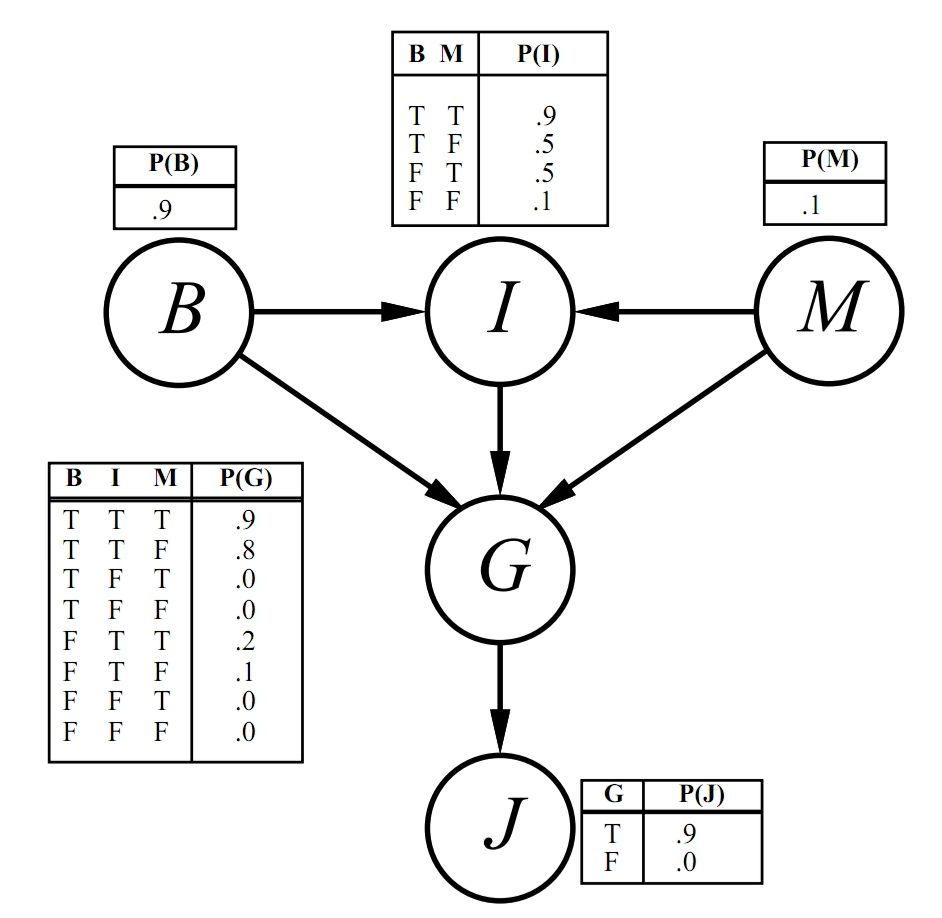
\includegraphics[scale=0.2]{fig14_23.jpg}
  \caption{A simple Bayes net with Boolean variables $B =
    BrokeElectionLaw, I = Indicted, M =
    PoliticallyMotivatedProsecutor, G = FoundGuilty, J = Jailed$. }
  \label{fig:2}
\end{figure}

\begin{enumerate}[a.]
\item Which of the following are asserted by the network structure?
\begin{enumerate}[i.]
\item $ P(B,I,M)=P(B)P(I)P(M) $.
\item $ P(J|G)=P(J|G,I) $.
\item $ P(M|G,B,I)=P(M|G,B,I,J) $. 
\end{enumerate}
\solution{$(ii) \mbox{ and } (iii) $ will be asserted by the network. \\
  For $(i)$, node B and M have the common effect of I. So, $P(B,I,M) =
  P(B)P(M)P(I|B,M)$. \\
  For $(ii)$, I, G and J has causal chain structure, so when G is given
  I and J will be independent, which is $P(J|G)=P(J|G,I)$. \\ 
  For $(iii)$, there exists two path from M to J, one is $M\rightarrow
  I\rightarrow G\rightarrow J$ and $M\rightarrow G\rightarrow J$. And
  both are causal chain structure, so when G is given M and J will be
  independent, that is $P(M|G,B,I)=P(M|G,B,I,J)$.
}

\item Calculate the value of $P(b, i, \neg m, g, j)$.
\solution{Using the Bayesian Network joint probability rule, we have 
\begin{eqnarray*}
  P(i) & = & P(i|b,m)P(b)P(m) + P(i|\neg b,m)P(\neg b)P(m) \\
  & + & P(i|b,\neg m)P(b)p(\neg m) + P(i|\neg b,\neg m)P(\neg b,\neg
  m) \\
  & = & 0.9*0.9*0.1 + 0.5*0.1*0.1 + 0.5*0.9*0.9 + 0.1*0.1*0.9 \\
  & = & 0.081 + 0.005 + 0.405 + 0.009 \\
  & = & 0.5 \\
  P(b, i, \neg m, g, j) & = & P(b)P(\neg m)P(i|b,\neg m)P(g|b,i,\neg
  m)P(j|g) \\
  & = & P(i)P(g|b,i,\neg m)P(j|g) \\
  & = & 0.5 \times 0.8 \times 0.9 \\
  & = & 0.36 
\end{eqnarray*}
}
\item Calculate the probability that someone goes to jail given that
  they broke the law, have been indicted, and face a politically
  motivated prosecutor.
\solution{We need to calculate $P(J|B,I,M)$. \\
  \begin{eqnarray*}
    P(I) & = & P(\neg I) = 0.5 \\
    P(G|B,I,M) & = & 0.9 \\ 
    P(G) & = & 0.37 \\
    P(J) & = & 0.396 \\
    P(J|B,I,M) & = & \frac{P(J|B,I,M)P(G|J)}{P(G|J)} \\
    & = & \frac{P(G,J|B,I,M)}{P(G|J)} \\ 
    & = & \frac{P(J|B,I,M,G)P(G|B,I,M)}{P(G|J)} \\
    & = & \frac{P(J|G)P(G|B,I,M)}{P(G|J)} (B,I,M\independent{J|G}) \\
    & = & \frac{P(J)P(G|B,I,M)}{P(G)} \\
    & = & \frac{0.396\times 0.9}{0.37} \\
    & = & 0.963 
  \end{eqnarray*}
}
\item A \textbf{context-specific independence} (see page 542) allows a
  variable to be independent of some of its parents given certain
  values of others. In addition to the usual conditional independences
  given by the graph structure, what context-specific independences
  exist in the Bayes net in Figure \ref{fig:2}?
  \solution{$
J\independent{B|G} \\
J\independent{I|G} \\
J\independent{M|G} \\
B\independent{M}
$}
\item Suppose we want to add the variable P =  PresidentialPardon the
network; draw the new network and briefly explain any links you add.
\solution{Please see the new Bayesian Network in Figure \ref{fig:14_14}.
  \begin{figure}[ht]
    \centering
    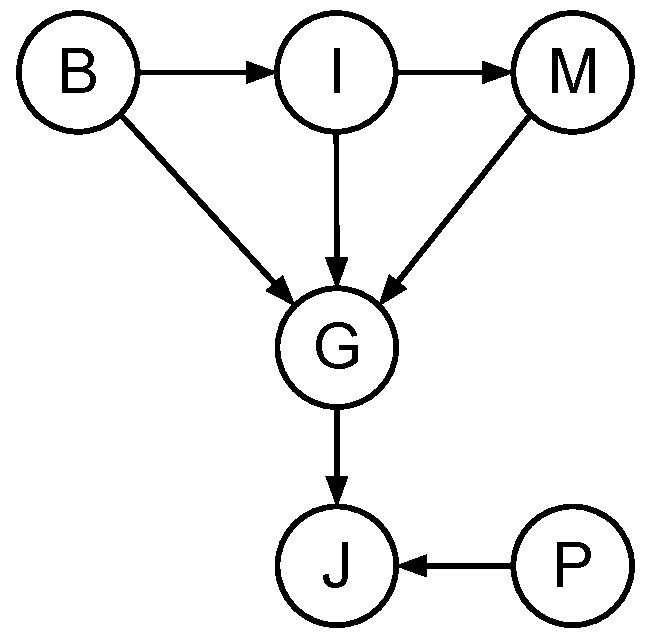
\includegraphics[width=.3\textwidth]{AI-HWK-2_14_14.pdf}
    \caption{Bayesian Network with PresidentialPardon.}\label{fig:14_14}
  \end{figure}
  In Figure \ref{fig:14_14}, node P is added as parent of J, because
  presendential pardon will only have direct influence on J, which is
  when a person is jailed. And other factors will not be affected by
  it. 
}
\end{enumerate}
\section{Execise 14.2}
Equation (14.1) on page 513 defines the joint distribution represented
by a Bayesian network in terms of the parameters $\theta
(X_i|Parents(X_i))$. This exercise asks you to derive the 
equivalence between the parameters and the conditional probabilities
$P(X_i|Parents(X_i))$ from this definition.
\begin{enumerate}[a.]
\item Consider a simple network $X \rightarrow Y \rightarrow Z$ with three
  Boolean variables. Use Equations (13.3) and (13.6) (pages 485 and
  492) to express the conditional probability $P(z|y)$ as the ratio of
  two sums, each over entries in the joint distribution $P(X,Y,Z)$. 
  \solution{
    Equation 13.3 : $P(a|b)=\frac{P(a,b)}{P(b)}$ and 
    Equation 13.6 : $P(Y)=\sum_zP(Y,z)$. \\
    The simple network tells us that $X\independent{Z}|Y$, which means
    $P(X,Z|Y) = P(X|Y)P(Z|Y)$. \\ 
    Based on knowledge above, we have:
    \[ P(z|y) = \frac{P(z,y)}{P(y)} =
    \frac{\sum_xP(x,y,z)}{\sum_x\sum_zP(x,y,z)}.\]
  }
\item Now use Equation (14.1) to write this expression in terms of the
  network parameters $\theta (X), \theta (Y|X)$, and $\theta(Z|Y)$.
  \solution{Equation 14.1 says:
    $P(x_1,x_2,\ldots,x_n)=\prod_{i=1}^n\theta (x_i|parent(x_i))$. \\
    And \[ \frac{\sum_xP(x,y,z)}{\sum_x\sum_zP(x,y,z)} =
    \frac{\sum_x\theta(x)\theta(y|x)\theta(z|y)} 
    {\sum_x\sum_z\theta(x)\theta(y|x)\theta(z|y)} \]
  }
\item Next, expand out the summations in your expression from part
  (b), writing out explicitly the terms for the true and false values
  of each summed variable. Assuming that all network parameters
  satisfy the constraint $\sum_{x_i}\theta (x_i|parents(X_i))=1$, show
  that the resulting expression reduces to \sout{$\theta(x|y)$}, (I
  think here should be $\theta(z|y)$). 
  \solution{
    First, we have $\sum_x\theta(x) = 1$ and
    $\sum_x\sum_z\theta(x)\theta(z|y) = 1\times 1 = 1$. \\
    So, 
    \[ \frac{\sum_x\theta(x)\theta(y|x)\theta(z|y)} 
    {\sum_x\sum_z\theta(x)\theta(y|x)\theta(z|y)} = 
    \frac{\theta(y|x)\theta(z|y)}{\theta(y|x)} = \theta(z|y).\]
}
\item Generalize this derivation to show that $\theta
  (X_i|Parents(X_i))=P(X_i|Parents(X_i))$ for any Bayesian network.
  \solution{In any Bayesian Network, the joint probability can be
    represented with $P(x_1,x_2,\ldots,x_n)=
    \prod_{i=1}^n\theta(x_i|parents(x_i))$, which is Equation 14.1. 
    And according to the joint probability theorem and the
    independence property in Bayesian networks, we can also write the
    joint probability of network variables as
    $\prod_{i=1}^nP(x_i|parents(x_i))$.
    So, it is easy to observe that $\theta
    (X_i|Parents(X_i))=P(X_i|Parents(X_i))$. 
}
\end{enumerate}
\section{Execise 14.7}
The Markov blanket of a variable is defined on page 517. Prove that a
variable is independent of all other variables in the network, given
its Markov blanket and derive Equation (14.12) (page 538).

\[ P(x_i^{\prime}|mb(X_i))=\alpha P(x_i^{\prime}|parents(X_i))\times
\prod_{y_j\in Children(X_i)}P(y_j|parents(Y_j)) \]
\solution{
\begin{proof}
  According to the theorem of d-speration and topological independence
  theorem, and simply considering the polytree structure of a Bayesian
  Network, we have the folloiwng assertions: \\
  \[ P(x_i|ancestors(X_i)) = P(x_i|parents(X_i)) \] which says $X_i$
  will be independent of its other ancestor nodes given its parents. 

  If given children of $X_i$, then for any decendents of
  $Children(X_i)$, we have:
  \[ P(x_i|decendents(X_i)) = P(x_i|children(X_i)) \] 
  
  If a node is connected with $X_i$ through $v$ structure with
  $Children(X_i)$ as mid-point, then we have 
  \[ P(x_i|decendents(X_i) =
  P(x_i|children(X_i),(parents(children(X_i))-X_i)) \]

  If for a node $X_j$, there is no path between $X_i$ and $X_j$. then
  they are simply independent. 

  All the four cases above covers all possible relationships between a
  node and another different node. And generalize the polytree
  structure to a directed acyclic graph (DAG) structure, in which
  case, there can be multiple paths between node $X_i$ and any other
  node. And by denoting Markov Blanket as 
  \[ MB(X_i)=parents(X_i)\cup children(X_i) \cup [parents(children(X_i))-X_i] \]
  we have that a variable is independent of all other variables given
  its Markov Blanket. 

  And \[P(x_i^{\prime}|mb(X_i))=\alpha P(x_i^{\prime}|parents(X_i))\times
  \prod_{y_j\in Children(X_i)}P(y_j|parents(Y_j)). \] 

\end{proof}
}

\end{document}